% Hedge Fund Pitch Deck — edit & compile online at https://letx.app
% Crestview Capital | NXSC Long Pitch | Q3 2026
\documentclass[10pt,aspectratio=169]{beamer}
\usepackage{amsmath}
\usepackage[T1]{fontenc}
\usepackage[utf8]{inputenc}
\usepackage{lato}
\renewcommand{\familydefault}{\sfdefault}
\usepackage{fontawesome5}
\usepackage{tikz}
\usepackage{pgfplots}
\pgfplotsset{compat=1.18}
\usepackage{tabularx}
\usepackage{booktabs}
\usepackage{array}
\usepackage[most]{tcolorbox}
\tcbuselibrary{skins,breakable}
\usetikzlibrary{shadows}
\usepackage{hyperref}
\usepackage{xcolor}
\usepackage{calc}

% ── Palette ──────────────────────────────────────────────────────────────────
\definecolor{navy}{HTML}{0A1F3F}
\definecolor{dnavy}{HTML}{061428}
\definecolor{gold}{HTML}{C8963E}
\definecolor{lgray}{HTML}{F4F5F7}
\definecolor{mgray}{HTML}{D5D8DC}
\definecolor{dtext}{HTML}{1E1E1E}
\definecolor{danger}{HTML}{C0392B}
\definecolor{profit}{HTML}{1E8449}
\definecolor{accentb}{HTML}{2980B9}

\setlength{\parindent}{0pt}
\setlength{\parskip}{0pt}

% ── Beamer templates ─────────────────────────────────────────────────────────
\setbeamertemplate{navigation symbols}{}

\setbeamertemplate{headline}{%
  
\begin{tikzpicture}[remember picture, overlay]
    \fill[navy] (0,0) rectangle (\paperwidth, 2.4pt);
  \end{tikzpicture}%
  \vspace{6pt}%
}

\setbeamertemplate{footline}{%
  \hspace{12pt}%
  \textcolor{mgray!70!white}{\rule{0.7pt}{10pt}}\hspace{8pt}%
  \textcolor{mgray!70!white}{\footnotesize\bfseries Crestview Capital}%
  \hfill%
  \textcolor{mgray!70!white}{\footnotesize\insertframenumber}%
  \hspace{16pt}%
  \vspace{8pt}%
}

\setbeamertemplate{frametitle}{%
  \vspace{4pt}%
  {\color{navy}\Large\bfseries\insertframetitle}%
  \vspace{2pt}%
  \par%
  \textcolor{gold}{\rule{28pt}{2pt}}%
  \vspace{6pt}%
}

\setbeamercolor{block title}{fg=white,bg=navy}
\setbeamercolor{block body}{fg=dtext,bg=lgray}
\setbeamercolor{block title example}{fg=white,bg=profit}
\setbeamercolor{block body example}{fg=dtext,bg=lgray}
\setbeamercolor{block title alerted}{fg=white,bg=danger}
\setbeamercolor{block body alerted}{fg=dtext,bg=lgray}

\setbeamerfont{frametitle}{series=\bfseries,size=\Large}
\setbeamerfont{block title}{series=\bfseries}

% ── Custom boxes ─────────────────────────────────────────────────────────────
\newtcolorbox{statbox}{
  colback=navy,coltext=white,boxrule=0pt,arc=4pt,
  left=12pt,right=12pt,top=8pt,bottom=8pt
}

\newtcolorbox{calloutbox}{
  colback=lgray,colframe=gold,boxrule=1.2pt,arc=3pt,
  left=10pt,right=10pt,top=6pt,bottom=6pt,
  before skip=8pt,after skip=8pt
}

\newtcolorbox{watermarkbox}{
  colback=navy!5,colframe=navy!30,boxrule=0.8pt,arc=2pt,
  left=10pt,right=10pt,top=6pt,bottom=6pt
}

% ── Helper macros ────────────────────────────────────────────────────────────
\newcommand{\kpi}[2]{%
  \begin{minipage}[t]{0.23\linewidth}
    \centering
    {\color{navy}\Large\bfseries #1}\\[2pt]
    {\color{dtext!70}\footnotesize #2}
  \end{minipage}%
}

\newcommand{\thesispoint}[2]{%
  \begin{minipage}[t]{0.48\linewidth}
    {\color{gold}\Large\faCaretRight}\hspace{6pt}%
    \begin{minipage}[t]{0.80\linewidth}
      {\color{navy}\bfseries #1}\\[2pt]
      {\footnotesize\color{dtext!80}#2}
    \end{minipage}
  \end{minipage}%
}

\newcommand{\risklabel}[1]{%
  {\small\bfseries\color{#1}\rule{0.7pt}{10pt}\hspace{4pt}}%
}

\begin{document}

% ══════════════════════════════════════════════════════════════════════════════
% SLIDE 1 — TITLE
% ══════════════════════════════════════════════════════════════════════════════
{
\setbeamertemplate{headline}{}
\setbeamertemplate{footline}{}
\begin{frame}[plain]
  \begin{tikzpicture}[remember picture, overlay]
    \fill[navy] (current page.north west) rectangle
      ([xshift=\paperwidth,yshift=-0.58\paperheight]current page.north west);
    \fill[dnavy] (current page.north west) rectangle
      ([xshift=\paperwidth,yshift=-0.60\paperheight]current page.north west);
    \node[anchor=north west,white] at ([xshift=28pt,yshift=-18pt]current page.north west)
      {\footnotesize\faBuilding\hspace{5pt}CRESTVIEW CAPITAL MANAGEMENT};
    \node[anchor=north west,white,opacity=0.7] at ([xshift=28pt,yshift=-52pt]current page.north west)
      {\small Long Pitch\enspace\textbar\enspace Q3 2026};
    \node[anchor=north west,white] at ([xshift=28pt,yshift=-102pt]current page.north west){%
      \begin{minipage}{0.85\paperwidth}
        {\fontsize{22}{28}\bfseries Nexus Semiconductor Corp.}\\[6pt]
        {\large\textcolor{gold}{NXSC \textbar\ NYSE\enspace\textbar\enspace Semiconductors}}\\[10pt]
        {\normalsize\textcolor{white!80}{Initiating Coverage — Target \$72.00\quad$\mid$\quad Upside +71\%}}
      \end{minipage}%
    };
    \node[anchor=south east,white!60] at ([xshift=-22pt,yshift=22pt]current page.south east)
      {\scriptsize CONFIDENTIAL — For Qualified Investors Only};
    \node[anchor=north east,gold] at ([xshift=-32pt,yshift=-150pt]current page.north east)
      {\huge\faChartBar};
    \draw[gold,line width=0.6pt]
      ([xshift=28pt,yshift=-78pt]current page.north west) --
      ([xshift=140pt,yshift=-78pt]current page.north west);
  \end{tikzpicture}
\end{frame}
}

% ══════════════════════════════════════════════════════════════════════════════
% SLIDE 2 — INVESTMENT THESIS
% ══════════════════════════════════════════════════════════════════════════════
\begin{frame}{Investment Thesis}
  \vspace{-4pt}

  \begin{columns}[T,onlytextwidth]
    \column{0.62\textwidth}
      \vspace{6pt}
      \thesispoint{Cyclical Recovery at Inflection}{NAND/DRAM capex bottomed in H1 2026; Nexus holds 34\% share in etch-deposition tools exposed to the 3nm transition. Revenue trough confirmed at \$1.9B TTM.}

      \vspace{10pt}
      \thesispoint{Proprietary Technology Moat}{17 years of process IP in high-aspect-ratio etching. Only two qualified vendors for TSMC N3 — switching costs exceed \$400M per fab line.}

      \vspace{10pt}
      \thesispoint{Margin Expansion Underway}{Gross margins troughed at 44.2\%; operating leverage on volume recovery drives 490 bps expansion to 49.1\% by FY2028E. SG\&A already right-sized.}

      \vspace{10pt}
      \thesispoint{Sum-of-Parts Undervalued}{Service recurring revenue (\$620M ARR) alone worth \$31/share on SaaS comps. Implies the equipment business trades at 7.2x EBITDA — a 10-year low.}

    \column{0.38\textwidth}
      \vspace{8pt}
      \begin{statbox}
        \centering
        {\footnotesize KEY METRICS}\\[6pt]
        {\fontsize{18}{22}\bfseries\$42.50}\\[1pt]
        {\footnotesize Current Price}\\[10pt]
        \textcolor{gold}{\rule{40pt}{0.6pt}}\\[8pt]
        {\fontsize{13}{16}\bfseries 71\%}\\[1pt]
        {\footnotesize Upside to Target}\\[10pt]
        \textcolor{gold}{\rule{40pt}{0.6pt}}\\[8pt]
        {\fontsize{13}{16}\bfseries 7.2$\times$}\\[1pt]
        {\footnotesize EV/EBITDA (ex-Services)}
      \end{statbox}

      \vspace{8pt}
      \begin{calloutbox}
        \centering
        {\footnotesize\bfseries\color{navy}Position Size Target}\\[2pt]
        {\color{dtext}\scriptsize 6.5\% of Fund NAV \textbar\ Entry \$40–\$44}
      \end{calloutbox}
  \end{columns}

\end{frame}

% ══════════════════════════════════════════════════════════════════════════════
% SLIDE 3 — COMPANY OVERVIEW & FINANCIALS
% ══════════════════════════════════════════════════════════════════════════════
\begin{frame}{Company Overview \& Key Financials}

  \vspace{-2pt}
  \begin{columns}[T,onlytextwidth]
    \column{0.45\textwidth}
      {\color{navy}\bfseries\small Business Description}\\[4pt]
      {\footnotesize\color{dtext!80}
      Nexus Semiconductor Corp. designs and manufactures plasma-etch and
      chemical-vapor-deposition tools for leading-edge logic and memory fabs.
      Headquartered in Boise, ID. 4,800 employees across 7 facilities in the US,
      Taiwan, and Singapore.}

      \vspace{8pt}
      {\color{navy}\bfseries\small Revenue Mix (TTM)}\\[4pt]
      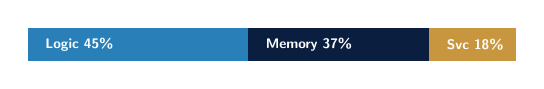
\begin{tikzpicture}
        \fill[accentb] (0,0) rectangle (2.8,0.42);
        \fill[navy] (2.8,0) rectangle (5.1,0.42);
        \fill[gold] (5.1,0) rectangle (6.2,0.42);
        \node[anchor=west,white,font=\tiny\bfseries] at (0.1,0.21) {Logic 45\%};
        \node[anchor=west,white,font=\tiny\bfseries] at (2.9,0.21) {Memory 37\%};
        \node[anchor=west,white,font=\tiny\bfseries] at (5.2,0.21) {Svc 18\%};
      \end{tikzpicture}

    \column{0.55\textwidth}
      {\color{navy}\bfseries\small Snapshot}\\[4pt]
      \setlength{\tabcolsep}{0pt}
      \begin{tabularx}{\linewidth}{@{}>{\color{navy}\bfseries\footnotesize}l@{\hspace{7mm}}>{\raggedright\arraybackslash\footnotesize}X@{}}
        Ticker / Exchange       & NXSC \textbar\ NYSE \\
        Share Price             & \$42.50 \\
        52-Week Range           & \$31.20 — \$48.75 \\
        Market Capitalization   & \$8.2B \\
        Enterprise Value        & \$9.1B \\
        TTM Revenue             & \$1,903M \\
        TTM EBITDA              & \$527M \\
        TTM Gross Margin        & 44.2\% \\
        Net Debt / EBITDA       & 1.7$\times$ \\
        Dividend Yield          & 1.8\% \\
        Short Interest (\% FF)  & 8.4\% \\
      \end{tabularx}
  \end{columns}

  \vspace{6pt}
  \begin{watermarkbox}
    \centering
    \kpi{\$2,340M}{FY2027E Revenue}\hfill
    \kpi{\$672M}{FY2027E EBITDA}\hfill
    \kpi{28.7\%}{EBITDA Margin}\hfill
    \kpi{14.2$\times$}{Fwd EV/EBITDA}
  \end{watermarkbox}

\end{frame}

% ══════════════════════════════════════════════════════════════════════════════
% SLIDE 4 — CATALYST TIMELINE
% ══════════════════════════════════════════════════════════════════════════════
\begin{frame}{Catalyst Roadmap}

  \vspace{4pt}
  \begin{columns}[T,onlytextwidth]
    \column{0.50\textwidth}
      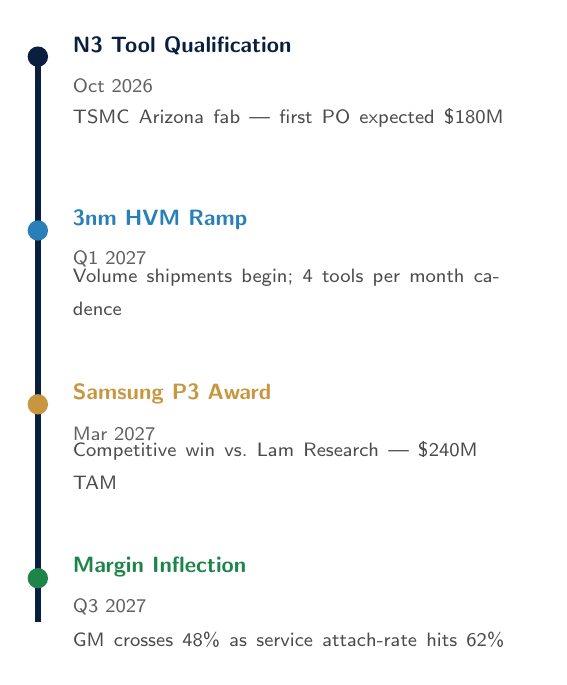
\begin{tikzpicture}[scale=0.92]
        \draw[navy,line width=2pt] (0,0) -- (0,-7.8);
        \foreach \y/\col/\label/\date/\detail in {
          0/navy/N3 Tool Qualification/Oct 2026/TSMC Arizona fab — first PO expected \$180M,
          -2.4/accentb/3nm HVM Ramp/Q1 2027/Volume shipments begin; 4 tools per month cadence,
          -4.8/gold/Samsung P3 Award/Mar 2027/Competitive win vs.\ Lam Research — \$240M TAM,
          -7.2/profit/Margin Inflection/Q3 2027/GM crosses 48\% as service attach-rate hits 62\%
        }{
          \fill[\col] (0,\y) circle (4pt);
          \node[anchor=west] at (0.35,\y+0.15) {{\footnotesize\bfseries\color{\col}\label}};
          \node[anchor=west] at (0.35,\y-0.40) {{\scriptsize\color{dtext!70}\date}};
          \node[anchor=west,text width=5.8cm] at (0.35,\y-0.85)
            {{\scriptsize\color{dtext!80}\detail}};
        }
      \end{tikzpicture}

    \column{0.50\textwidth}
      \vspace{8pt}
      \begin{calloutbox}
        {\footnotesize\bfseries\color{navy}Revenue Cadence Bridge}\\[4pt]
        \setlength{\tabcolsep}{0pt}
        \begin{tabularx}{\linewidth}{@{}>{\color{navy}\bfseries\footnotesize}l@{\hspace{5mm}}>{\raggedright\arraybackslash\footnotesize}X@{}}
          FY2026E & \$1,910M\enspace{\color{dtext!50}\scriptsize(flat)}\\
          FY2027E & \$2,340M\enspace{\color{profit}\scriptsize+23\%}\\
          FY2028E & \$2,810M\enspace{\color{profit}\scriptsize+20\%}\\
        \end{tabularx}
      \end{calloutbox}

      \vspace{6pt}
      \begin{block}{}
        \centering
        {\footnotesize\bfseries\color{navy}Key Inflection Point}\\[4pt]
        {\small TSMC N3 represents the largest node transition since 7nm in 2018.}
        {\small Nexus is sole-sourced on 4 of 7 critical etch steps.}
      \end{block}

      \vspace{6pt}
      {\footnotesize\color{dtext!70}\faExclamationTriangle\hspace{4pt}Risk: Texas Instruments pulled in-sourcing timeline to H2 2027 — could accelerate Nexus bookings by 1–2 quarters.}
  \end{columns}

\end{frame}

% ══════════════════════════════════════════════════════════════════════════════
% SLIDE 5 — VALUATION WATERFALL
% ══════════════════════════════════════════════════════════════════════════════
\begin{frame}{Valuation Waterfall}
  \vspace{-4pt}

  \begin{columns}[T,onlytextwidth]
    \column{0.52\textwidth}
      \vspace{8pt}
      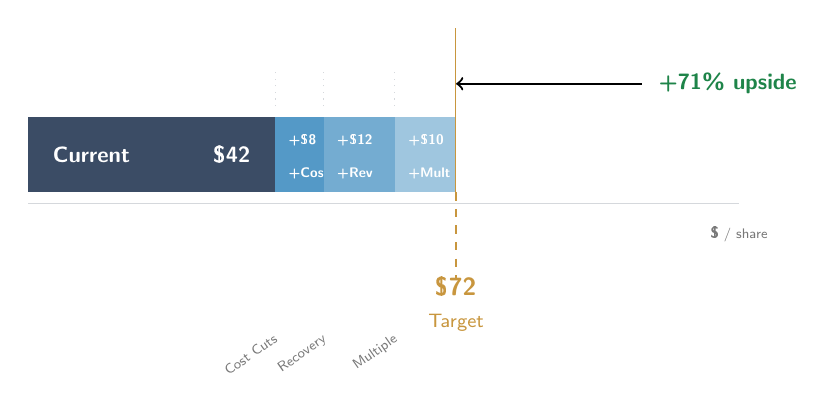
\begin{tikzpicture}[scale=0.95]
        \draw[mgray,line width=0.4pt] (0,0) -- (9.5,0);
        \node[anchor=north,font=\tiny\color{dtext!60}] at (9.5,-0.2) {\$ / share};

        % Current
        \fill[navy!80] (0,0.15) rectangle (3.3,1.15);
        \node[anchor=west,white,font=\footnotesize\bfseries] at (0.2,0.65) {Current};
        \node[anchor=east,white,font=\footnotesize\bfseries] at (3.1,0.65) {\$42};

        % + Cost restructuring
        \fill[accentb!80] (3.3,0.15) rectangle (3.95,1.15);
        \node[anchor=west,white,font=\tiny\bfseries] at (3.35,0.40) {+Cost};
        \node[anchor=west,white,font=\tiny\bfseries] at (3.35,0.85) {+\$8};

        % + Revenue recovery
        \fill[accentb!65] (3.95,0.15) rectangle (4.90,1.15);
        \node[anchor=west,white,font=\tiny\bfseries] at (4.0,0.40) {+Rev};
        \node[anchor=west,white,font=\tiny\bfseries] at (4.0,0.85) {+\$12};

        % + Multiple expansion
        \fill[accentb!45] (4.90,0.15) rectangle (5.70,1.15);
        \node[anchor=west,white,font=\tiny\bfseries] at (4.95,0.40) {+Mult};
        \node[anchor=west,white,font=\tiny\bfseries] at (4.95,0.85) {+\$10};

        % Target bar spanning full width to $72
        \fill[gold] (5.70,0.15) rectangle (5.72,2.35);
        \draw[gold,dashed,line width=1pt] (5.72,0.15) -- (5.72,-1.0);
        \node[anchor=north,gold,font=\small\bfseries] at (5.72,-0.85) {\$72};
        \node[anchor=north,gold,font=\scriptsize] at (5.72,-1.35) {Target};

        % Uspide annotation
        \draw[<-,line width=0.8pt] (5.72,1.6) -- (8.2,1.6);
        \node[anchor=west] at (8.3,1.6) {{\footnotesize\bfseries\color{profit}+71\% upside}};

        % Dotted line from current to start of bars
        \draw[mgray,dotted] (3.3,1.3) -- (3.3,1.8);
        \draw[mgray,dotted] (3.95,1.3) -- (3.95,1.8);
        \draw[mgray,dotted] (4.90,1.3) -- (4.90,1.8);

        % Bottom axis labels
        \node[font=\tiny\color{dtext!60},rotate=35,anchor=north east] at (3.3,-1.55) {Cost Cuts};
        \node[font=\tiny\color{dtext!60},rotate=35,anchor=north east] at (3.95,-1.55) {Recovery};
        \node[font=\tiny\color{dtext!60},rotate=35,anchor=north east] at (4.90,-1.55) {Multiple};
      \end{tikzpicture}

    \column{0.48\textwidth}
      \vspace{10pt}
      {\color{navy}\bfseries\small Methodology}\\[6pt]
      \begin{tabularx}{\linewidth}{@{}>{\color{navy}\bfseries\footnotesize}l@{\hspace{5mm}}>{\raggedright\arraybackslash\footnotesize}X@{\hspace{2mm}}r@{}}
        DCF (8.5\% WACC)          & 5-year explicit, 2.5\% terminal & \color{profit}\bfseries\$74 \\
        EV/EBITDA Comps           & 16.0$\times$ FY2027E (peer median) & \color{profit}\bfseries\$70 \\
        SOTP — Services           & 5.5$\times$ recurring rev at 42\% margin & \color{profit}\bfseries\$31 \\
        SOTP — Equipment          & 10.0$\times$ FY2027E EBITDA & \color{profit}\bfseries\$38 \\
        \cmidrule{3-3}
        \textbf{Probability-Weighted} & \textbf{40\% Base / 35\% Bull / 25\% Bear} & \color{profit}\bfseries\$72 \\
      \end{tabularx}

      \vspace{6pt}
      \begin{calloutbox}
        \centering
        {\footnotesize\bfseries\color{navy}Scenario Analysis}\\[4pt]
        \begin{tabularx}{\linewidth}{@{}>{\footnotesize}l@{\hspace{4mm}}>{\centering\arraybackslash\footnotesize}X@{\hspace{4mm}}>{\centering\arraybackslash\footnotesize}X@{\hspace{4mm}}>{\centering\arraybackslash\footnotesize}X@{}}
                         & Bear      & Base      & Bull \\
          Price Target   & \$28      & \$65      & \$95 \\
          Upside         & {\color{danger}-34\%} & {\color{profit}+53\%} & {\color{profit}+124\%} \\
          EV/EBITDA      & 6.0$\times$ & 14.0$\times$ & 18.0$\times$ \\
        \end{tabularx}
      \end{calloutbox}

      \vspace{4pt}
      {\footnotesize\color{dtext!70}\faLightbulb\hspace{4pt} Bear case assumes delayed 3nm ramp + TI fab cancellation. Bull case assumes sole-source win at Intel 18A.}
  \end{columns}

\end{frame}

% ══════════════════════════════════════════════════════════════════════════════
% SLIDE 6 — RISK MATRIX
% ══════════════════════════════════════════════════════════════════════════════
\begin{frame}{Risk Matrix \& Position Management}
  \vspace{-2pt}

  \begin{tabularx}{\linewidth}{@{}>{\raggedright\arraybackslash\footnotesize}X@{\hspace{4mm}}c@{\hspace{4mm}}c@{\hspace{4mm}}>{\raggedright\arraybackslash\footnotesize}X@{}}
    \toprule
    \textcolor{navy}{\bfseries\small Risk}
      & \textcolor{navy}{\bfseries\small Severity}
      & \textcolor{navy}{\bfseries\small Prob.}
      & \textcolor{navy}{\bfseries\small Mitigation} \\
    \midrule
    Delayed 3nm customer qualification &
      \risklabel{danger}High & 25\% &
      Hedge with sector puts; monitor TSMC capex guidance monthly. \\
    \addlinespace[3pt]
    Memory cycle downturn extends beyond Q4 2026 &
      \risklabel{danger}High & 15\% &
      Service revenue (\$620M ARR) provides floor; 1.8\% dividend yield cushions. \\
    \addlinespace[3pt]
    Competitor (Lam Research) wins N3 process steps &
      \risklabel{gold}Med & 20\% &
      Switching costs exceed \$400M; Nexus holds 17-year process qualification history. \\
    \addlinespace[3pt]
    Geopolitical — Taiwan Strait escalation &
      \risklabel{danger}High & 10\% &
      Arizona fab (online late-2026) de-risks single-point exposure to Hsinchu. \\
    \addlinespace[3pt]
    Customer consolidation (SK Hynix + Samsung merger) &
      \risklabel{accentb}Low & 5\% &
      Nexus diversified across 14 customers; top-3 = 48\% of revenue. \\
    \bottomrule
  \end{tabularx}

  \vspace{8pt}
  \begin{columns}[T,onlytextwidth]
    \column{0.50\textwidth}
      \begin{block}{Position Sizing Framework}
        \centering
        \begin{tabularx}{\linewidth}{@{}>{\footnotesize\bfseries\color{navy}}l@{\hspace{5mm}}>{\centering\arraybackslash\footnotesize}X@{}}
          Entry Zone       & \$40 — \$44 \\
          Max Position     & 6.5\% NAV \\
          Stop-Loss        & \$31 (-27\%) \\
          Take-Profit      & \$72 (+71\%) \\
          Reward/Risk      & 2.6 : 1 \\
        \end{tabularx}
      \end{block}

    \column{0.50\textwidth}
      \begin{alertblock}{Key Monitor Items}
        {\footnotesize
        \faCheckSquare\hspace{4pt} TSMC monthly revenue (10th of each month)\\[3pt]
        \faCheckSquare\hspace{4pt} SEMI book-to-bill ratio\\[3pt]
        \faCheckSquare\hspace{4pt} Q4 2026 earnings (Jan 28, 2027)\\[3pt]
        \faCheckSquare\hspace{4pt} Samsung P3 tool award (Q1 2027)
        }
      \end{alertblock}
  \end{columns}

\end{frame}

% ══════════════════════════════════════════════════════════════════════════════
% SLIDE 7 — SUMMARY & RECOMMENDATION
% ══════════════════════════════════════════════════════════════════════════════
\begin{frame}{Summary \& Recommendation}

  \vspace{2pt}
  \begin{columns}[T,onlytextwidth]
    \column{0.58\textwidth}
      \begin{block}{}
        \begin{itemize}
          \setlength{\itemsep}{3pt}
          \item[\color{gold}\faCheckCircle] {\footnotesize\bfseries Cyclical trough with 3 visible catalysts over 12 months}
          \item[\color{gold}\faCheckCircle] {\footnotesize\bfseries Technology moat validated by TSMC sole-source at N3}
          \item[\color{gold}\faCheckCircle] {\footnotesize\bfseries 490 bps of margin expansion embedded in base case}
          \item[\color{gold}\faCheckCircle] {\footnotesize\bfseries SOTP implies equipment business at 10-year trough multiple}
          \item[\color{gold}\faCheckCircle] {\footnotesize\bfseries 2.6:1 reward/risk with defined stop-loss discipline}
        \end{itemize}
      \end{block}

    \column{0.42\textwidth}
      \begin{statbox}
        \centering
        {\footnotesize RECOMMENDATION}\\[4pt]
        {\fontsize{18}{22}\bfseries\color{gold}BUY}\\[2pt]
        {\footnotesize NXSC — Long Only}\\[8pt]
        \textcolor{white!60}{\rule{40pt}{0.5pt}}\\[6pt]
        {\normalsize\bfseries Target: \$72.00}\\[1pt]
        {\small Upside: +71\%}\\[1pt]
        {\footnotesize Horizon: 12–18 months}
      \end{statbox}

      \vspace{4pt}
      \begin{calloutbox}
        \centering
        {\footnotesize\bfseries\color{navy}Portfolio Fit}\\[1pt]
        {\scriptsize Cyclical value with hard catalyst path.\quad Corr. to SPX: 0.41}
      \end{calloutbox}
  \end{columns}

  \begin{tikzpicture}[remember picture, overlay]
    \fill[navy] (current page.south west) rectangle
      ([xshift=\paperwidth,yshift=16pt]current page.south west);
    \node[anchor=west,white,font=\tiny\bfseries] at
      ([xshift=28pt,yshift=8pt]current page.south west)
      {Crestview Capital Management\enspace\textbar\enspace
       \faEnvelope\enspace ir@crestviewcap.com\enspace\textbar\enspace
       \faPhone\enspace (212) 555-0147};
  \end{tikzpicture}

\end{frame}

\end{document}
